% This is a default-selection of plugins that are used widely in this repo.

\documentclass[a4paper,10pt,fleqn]{article}
\usepackage[utf8]{inputenc}

% deutsche Trennmuster etc.
\usepackage[ngerman]{babel}
\usepackage[T1]{fontenc}

% mathematical simbols and fonts
\usepackage{mathtools} 
\usepackage{amssymb}
\usepackage{amsmath}
\usepackage{ntheorem}
\usepackage{polynom}
\usepackage{marvosym}
\usepackage{tabu}
\renewcommand*{\bmod}{\mathbin{\%}}
\everymath{\displaystyle}

\usepackage{multicol}
\usepackage{color}
\usepackage[usenames,dvipsnames]{xcolor}
\setlength{\columnsep}{1cm}
\setlength{\columnseprule}{0.25pt}
\def\columnseprulecolor{\color{gray}}
\usepackage{hyperref}

\usepackage[margin=1.5cm]{geometry}
\usepackage{graphicx}
\usepackage{pgfplots}
\pgfplotsset{compat=1.10}

%Code higlighting

\usepackage{minted}

% make lists more compact:
\newlength{\wideitemsep}
\setlength{\wideitemsep}{.5\itemsep}
\addtolength{\wideitemsep}{-5pt}
\let\olditem\item
\renewcommand{\item}{\setlength{\itemsep}{\wideitemsep}\olditem}
\renewcommand{\arraystretch}{1.25}

\title{Zusammenfassung CN2}
\author{Fabian Hauser}
 
\begin{document}
\maketitle

\section{Varia}
10 Seiten A4 Zusammenfassung

\section{Telefonie}

\begin{description}
\item[Data Plane] \hfill \\
	Forward IP-Packets. Z.B. STP, VLANs
\item[Control Plane] \hfill \\
	Routing Protocols, Overlay technologies (MPLS), z.B: Forwarding of Ethernet Frames
\end{description}


\subsection{G.711 / PCM}
 256 Audio-Steps using 8 Bits, Sample 8000/sec (nyquist frequency) = DS0, 64Kbps


\subsection{ISDN}
Braucht NT Wandler.

\begin{description}
\item[S-Bus] \hfill \\
	 Digitaler Bus im Haus; Data Plane.
\item[D-Kanal] \hfill \\
	Synchronisierungs-Kanal zur Dorfzentrale
\item[PBX] \hfill \\
	Die Dorfzentrale; Übersetzt Rufnummer-Anfragen (Wählton) zu weiteren Zentralen

\end{description}

\subsection{SS7}

Ähnlich BGP ist das SS7 Routing Protokoll die Verbindung zwischen allen Telefonzentralen.
	
\subsection{Voip}
Läuft über Router; muss von Telefonnummer eine IP-Addresse "extrahieren".
	
\subsubsection{The Connection / Bearer Plane}
Switching Logic: Connection Negotiation, Transcoding

Mittels z.B. SIP mit CCP Verbunden.

\subsubsection{The Call Control Plane: SIP as a Example}
Call Logic: Signalling \& Call control
Logic / Services

Mittels z.B. TAPI / INAPI mit Services Plane verbunden.

Distributed call processing: (SIP, H.323), Centralized cal process (SCCP, MGCP, MEHACO, H.248)

Inititation von Verbindungen

\subsubsection{The Services Plane}
Service Logic: IN Service Logic, AAA, Address Resolution


\subsection{Session Description Protocol SDP}
Manage the Lines respectivly connection properties

\begin{description}
\item INVITE \hfill \\
	codecs support etc.
\item REGISTER
\item BYE
\item ACK 
\item CANCEL
\item OPTIONS
\end{description}

Mediaübertragung über RTP.

\subsection{SIP}

\begin{itemize}
	\item User location
	\item User availability
	\item User capabilies
	\item Session setup
	\item Session management
\end{itemize}

Makes use of:
\begin{itemize}
	\item HTTP
	\item SDP
	\item RTP / RTSP
	\item URI / URL
	\item DHCP / DNS
	\item MIME
	\item TLS / IPSec
\end{itemize}

\begin{description}
	\item Registrar Server \hfill \\
		Datase of IP / Numbers matching of the User Agent
	\item Proxy \hfill \\
		Routing of SIP signalling messages
	\item Redirect Server \hfill \\
		Redirects von Anrufen
\end{description}

\section{Routing}

Layer 3, dynamisch oder statisch

\subsection{Routing Hierarchy}

Separiert in \emph{Autonomous Systems} (AS). Zwischen den AS wird mit \emph{Exterior Routing Protocols} (EGP) benutzt, üblicherweise BGP.

Innerhalb der AS wird ein Interior routing Protocol (IGP) verwendet.

\subsection{Distance Vector}

Es wird jeweils die ganze Tabelle zurückgegeben.

\subsubsection{Split Horizon}

Der Router, welcher die Route mitgeteilt hat, wird nicht "wiederholt".

\subsection{Link State Protocol}

\begin{enumerate}
	\item Ermittlung Nachbarn mit Hello Protocol
	\item Kenntnisse Nachbarn weitergeben. (\emph{Link State Advertisments})
	\item \emph{Shortest Path First} nach kenntniss von ganzer Datenbank
\end{enumerate}

Es wir jeweils nur ein Single Entry durchgegeben, mit dem Inhalt (RouterID, NeighborID, Cost)

\subsubsection{Shortest Path Algorithm}

\begin{enumerate}
\item %TODO	
\end{enumerate}


\subsection{OSPF}

\begin{itemize}
	\item Secure (Signing)
	\item Classless
	\item Max 50 client per Area
\end{itemize}


\subsection{BGP}

Border Gateway Protocoll

\subsubsection{Autonomouse Systems}

1-65535 unique
private AS pool from 64512 to 65535 (similar to private IPs)
RFC 6793 introduces 32 bit AS numbers
(y.x), each x/y = 16bits
BGP4, is used to interconnect AS

\subsubsection{Connection}

\paragraph{Home} \hfill \\

Access to ISP; default route

\paragraph{Multi-Homed} \hfill \\
Connected with muliple AS Provider or multiple Links to the same Provider

\begin{description}
	\item[Transit AS] \hfill \\
	Can be used for transit traffic by other providers
	\item[Nontransit AS] \hfill \\
	Advertises only its own routes to both providers
\end{description}

\subsubsection{Protocol}

The less hops the better

Communicates in which AS are which IP Ranges.

BGP4 supports CIDR and route aggregation

BGP is a Path vector protocol

TCP Port 179

\begin{enumerate}
	\item OPEN MESSAGE: Exchange AS, router ID, holdtime, Capability negotiation
	\item NOTIFICATION (Example: ''peer in wrong AS'')
	\item KEEPALIVE when no updates
	\item UPDATE (incremental)
\end{enumerate}


Netze werden explizit Withdrwan

Attributes: Pfadlängen, Kosten etc.

Prefixes: Neuer Weg etc.

\subsubsection{Types}
(\emph{Nicht} zum auswendig-lernen)
\begin{description}
	\item[1: ORIGIN]
	\item[2: AS-PATH]
	\item[3: NEXT-HOP]
	\item[4: MED] Multi Exit Discriminator (Reccomandations Traffic ports)
	\item[5: LOCAL\_PREF] Local preferences
\end{description}

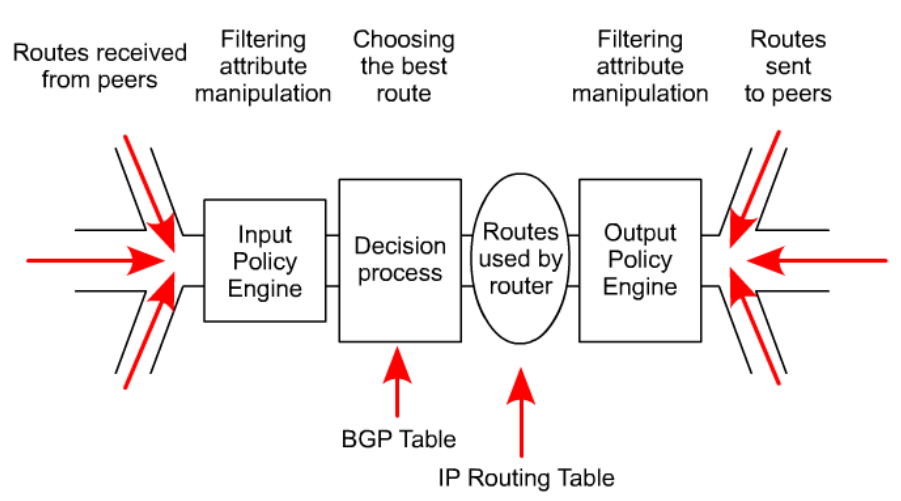
\includegraphics[width=0.5\linewidth]{img/bgp_process_model.png}

\subsubsection{Peering vs. Transit}

Transit: Kostet, quasi default gateway wo via peering nicht abgedeckt.
Peering: Lokale Provider verknüpfen. (üblicherweise Gratis).

\paragraph{Peering}
Multi-lateral Peering: Zentrale Einheit welche das Peering organisiert (Zentraler Swtich)

Bi-lateral Peering: Direktes Peering mit anderem Provider.



\end{document}